\documentclass[11pt]{article}
\usepackage[T1]{fontenc}
\usepackage[margin=1in]{geometry}
\usepackage{amsmath,amssymb}
\usepackage{graphicx}
\usepackage{booktabs}
\usepackage{array}
\usepackage{xcolor}
\usepackage[colorlinks=true,linkcolor=blue!60!black,urlcolor=blue!60!black]{hyperref}
\usepackage{listings}
\lstset{basicstyle=\ttfamily\small, backgroundcolor=\color{gray!8},
        frame=single, rulecolor=\color{gray!40}, breaklines=true,
        columns=fullflexible, keepspaces=true}

\newcommand{\code}[1]{\texttt{#1}}
\newcommand{\file}[1]{\texttt{#1}}
\newcommand{\Om}{\Omega}

\title{Dust Particles and Gas$+$Dust Self-Gravity\\
       in the AthenaK Shearing Box:\\
       I.\ The Dust-Module Merge (Phase 4a)}
\author{\code{athenak-multigrid} tree, branch \code{dust-multigrid}}
\date{September 3, 2026}

\begin{document}
\maketitle

\begin{abstract}
\noindent
This document opens the \emph{dust track} of the self-gravity program: Lagrangian
dust particles in the shearing-box code with multigrid self-gravity on refined
meshes, toward the gas$+$dust gravito-turbulent boxes of Baehr, Zhu \& Yang (2022)
with the radial pressure gradient they omitted. It records what the code does on
test problems, phase by phase; the mechanisms are in the companion
\file{dust\_selfgravity\_implementation.pdf}.

\textbf{Phase 4a} merges the sibling fork \code{athenak-dust} --- particle-mesh dust
with Benítez-Llambay--Krapp--Pessah implicit drag inside the Krapp et al.\ (2024)
IMEX integrator, validated in its own repository --- into the multigrid tree, and
asks two questions: is the dust module unchanged by the merge, and is the gravity
machinery unchanged by the dust module? Both answers are yes to every printed digit.
On the merged tree the dust fork's own acceptance numbers reproduce exactly: the
$N$-species damping ladder converges at second order in $\Delta t$ with the
reference errors $1.3529\times10^{-7}$, $3.4627\times10^{-8}$, $8.7724\times10^{-9}$,
$2.2075\times10^{-9}$ and total momentum conserved to $10^{-16}$; the multi-species
Nakagawa--Sekiya--Hayashi drift equilibrium holds to $10^{-16}$ over ten orbits; the
damped dusty sound wave converges toward second order in resolution; the ion-neutral
C-shock under \code{imex2+} is bit-identical to its baseline. The gravity solver's
documented statics reproduce exactly (slab sheet error $1.203\times10^{-12}$, Tomida
\& Stone contraction $0.125$, boundary-annuli shearing wave
$5.950\times10^{-3}$ / $2.057\times10^{-3}$), bit-identically at 4 ranks. The one
defect found --- a multi-rank deadlock of the additive deposit exchange against the
tree's rank-packed messaging --- is fixed and ranks 1, 2 and 4 agree to all digits.
Finally the gas-only stratified gravito-turbulence box evolved with \code{rk2} and
with \code{imex2+} (the integrator the dust module requires) agrees in every history
column to between $2\times10^{-6}$ and $5\times10^{-3}$ at $t = 3\,\Om^{-1}$, the
expected spread between two second-order integrators.

A \textbf{second merge} the same day brought in the dust fork's latest seven commits.
The whole battery reproduces on the result to every digit (the gas-only run bit for
bit), and the fork's new predictor--corrector coupling under plain \code{rk2}
(\code{coupling = pc2}) is exercised for the first time here: second order in the
damping ladder (orders $2.23$, $2.10$, $2.04$) and in the dusty wave ($1.85$, $1.98$,
$2.00$), NSH to round-off, rank-independent at 1, 2 and 4 ranks --- the integrator
freedom that lets dust run under the same \code{rk2} as every gravity result before it.
\end{abstract}

\tableofcontents
\newpage

%=========================================================================================
\section{Plan and scope}
\label{sec:plan}

\subsection{The program}

The science target is the interplay of gas gravitational instability and dust
concentration: 3D stratified, cooling, gravito-turbulent shearing boxes with
superparticles (Baehr, Zhu \& Yang 2022: $512^2\times256$, $\beta = 10$ cooling with an
irradiation floor, $\gamma = 5/3$, $\mathrm{St} = 0.1$, $1$, $10$, $Z = 0.01$,
$Q_0 = 1.02$), extended by the radial pressure gradient that admits the streaming
instability, and eventually adaptive zoom on the dust clumps --- the configuration
their limitations section names. The route (implementation document, \S1.2):
Phase 4a merges the dust module; 4b adds what the 3D shearing box needs from it
(shear-remapped additive deposits, ideal-gas back-reaction, a relaxed particle
timestep); 4c adds dust self-gravity through the existing Poisson solve; 4d builds
the science configuration; Phase 5 takes particles onto refined meshes.

\subsection{What Phase 4a must establish}

\begin{enumerate}\itemsep2pt
  \item \textbf{Dust fidelity.} The dust fork ships its validation in
        \file{../athenak\_dust\_tests/} (notebooks with printed reference values). On the
        merged tree, those references must reproduce: the damping ladder (second order in
        $\Delta t$, momentum to round-off), the NSH drift equilibrium (round-off over ten
        orbits), the damped dusty wave (spatial convergence), the random-placement and
        single-block layout checks, and the regression of the ion-neutral C-shock that
        shares the \code{imex2+} coefficient code.
  \item \textbf{Gravity regression.} Three static multigrid tests whose numbers are
        documented in the multigrid validation document: the slab-open sheet test, the
        Tomida \& Stone \S4.1 contraction, and the boundary-annuli shearing wave
        including its zero-phase bit-identity with the periodic twin.
  \item \textbf{Rank independence.} Dust and gravity at 1, 2 and 4 MPI ranks.
  \item \textbf{Integrator.} The dust module's IMEX coupling requires \code{imex2+};
        all gravity validation so far used \code{rk2}. A gas-only stratified
        gravito-turbulence box under both integrators, compared column by column.
  \item \textbf{The second merge} (\S\ref{sec:merge2}). After catching up with the dust
        fork: the battery again, and the new PC2/hybrid couplings under \code{rk2}.
\end{enumerate}

%=========================================================================================
\section{Test setup}
\label{sec:setup}

\subsection{Builds}

Serial and MPI builds in the tree's \file{build/} and \file{build-mpi/}, both with
\code{-D PROBLEM=built\_in\_pgens -D Athena\_ENABLE\_FFT=ON}, the MPI one with
\code{-D Athena\_ENABLE\_MPI=ON} (Open MPI via Homebrew). Everything below was first
run on a scratch clone at the same commits and then rerun with the tree's own
binaries; the two sets of results are identical, including the gravito-turbulence
histories bit for bit.

\subsection{Inputs and commands}

Dust inputs come from the dust-tests repository (paths relative to the directory
holding both trees):

\begin{lstlisting}
# damping ladder (tlim = 1, so dt = 1/ncycle)
for c in 0.4 0.2 0.1 0.05; do
  athena -i athenak_dust_tests/inputs/dust_damping.athinput particles/ppc=3 time/cfl_number=$c
done
# layout variants
athena -i .../dust_damping.athinput particles/ppc=4 problem/lattice=false
athena -i .../dust_damping.athinput particles/ppc=4 problem/lattice=false dust/deposit=ngp
athena -i .../dust_damping.athinput particles/ppc=3 meshblock/nx1=32 meshblock/nx2=32
# NSH equilibrium, dusty wave, C-shock regression
athena -i .../dust_nsh.athinput
athena -i .../dusty_wave.athinput mesh/nx1=$n meshblock/nx1=$((n/2))     # n = 32..256
athena -i inputs/ion-neutral/perp_cshock.athinput time/integrator=imex2+ time/nlim=500
# rank independence (drifting particles cross MeshBlock and rank boundaries)
mpirun -np $np athena -i .../dust_damping.athinput particles/ppc=3 problem/v0=0.5 dust/taus_3=0.5
# gravity statics
athena -i inputs/tests/mg_poisson_slab.athinput
athena -i inputs/tests/ts41_sin3.athinput
athena -i inputs/tests/mg_poisson_shear_bndry.athinput problem/profile=shwave problem/time0=0.37
# integrator twin (gas only, uniform grid)
athena -i inputs/shearing_box/gravito_turb_amr_test.athinput mesh_refinement/refinement=none \
       time/tlim=3.0 [time/integrator=imex2+ time/cfl_number=0.3]
\end{lstlisting}

Each dust problem generator writes a \file{<basename>-errs.dat} line per run; the
gravity statics print their metrics to standard output. All result files are
archived under \file{validation/run/dust4a/} (see its \file{README.txt}), which the
figure scripts \file{figures/plot\_dust4a\_*.jl} read.

%=========================================================================================
\section{Results}
\label{sec:results}

\subsection{Dust fidelity}
\label{sec:fidelity}

\paragraph{Damping ladder (Krapp et al.\ 2024 \S3.1).} Uniform gas at rest coupled
to three dust species, $t_s = (0.01, 0.1, 1.0)$, $\epsilon_s = 1/3$ each, one particle
of every species at every cell center so the discrete update per cell \emph{is} the
integrator's map of the ODE system. Errors are against a fine-step RK4 reference;
the first run has $\Delta t > t_{s,1}$ (stiff regime).

\begin{center}
\small
\begin{tabular}{@{}rccccc@{}}
\toprule
$\Delta t$ & err$_u$ & err$_{v1}$ & err$_{v2}$ & err$_{v3}$ & $|\Delta P_{\rm tot}|$ \\
\midrule
$1.235\times10^{-2}$ & $1.3529\times10^{-7}$ & $1.3711\times10^{-7}$ & $1.4641\times10^{-7}$ & $6.8939\times10^{-7}$ & $1.6\times10^{-16}$ \\
$6.211\times10^{-3}$ & $3.4627\times10^{-8}$ & $3.5096\times10^{-8}$ & $3.7325\times10^{-8}$ & $1.7630\times10^{-7}$ & $7.5\times10^{-17}$ \\
$3.115\times10^{-3}$ & $8.7724\times10^{-9}$ & $8.8920\times10^{-9}$ & $9.4213\times10^{-9}$ & $4.4631\times10^{-8}$ & $2.0\times10^{-16}$ \\
$1.558\times10^{-3}$ & $2.2075\times10^{-9}$ & $2.2377\times10^{-9}$ & $2.3649\times10^{-9}$ & $1.1225\times10^{-8}$ & $1.7\times10^{-16}$ \\
\midrule
order of err$_u$ & \multicolumn{5}{l}{$1.98$, $1.99$, $1.99$} \\
reference (dust tests, 2026-07-14) & \multicolumn{5}{l}{err$_u$ $= 1.3529\times10^{-7}$,
  $3.4627\times10^{-8}$, $8.7724\times10^{-9}$, $2.2075\times10^{-9}$; $|\Delta P| \sim 10^{-16}$} \\
\bottomrule
\end{tabular}
\end{center}

Every reference digit reproduces (Fig.~\ref{fig:damping}). The layout variants:
random positions with TSC and with NGP deposit give err$_u = 5.29\times10^{-6}$ and
$5.77\times10^{-6}$ (the $10^{-5}$-level departure from the homogeneous ODE is
physical: density fluctuations couple to pressure) with momentum to
$3.8\times10^{-16}$; the single-MeshBlock lattice run reproduces the four-block ladder
row to all digits, which is the halo-exchange exactness check.

\begin{figure}[htbp]
\centering
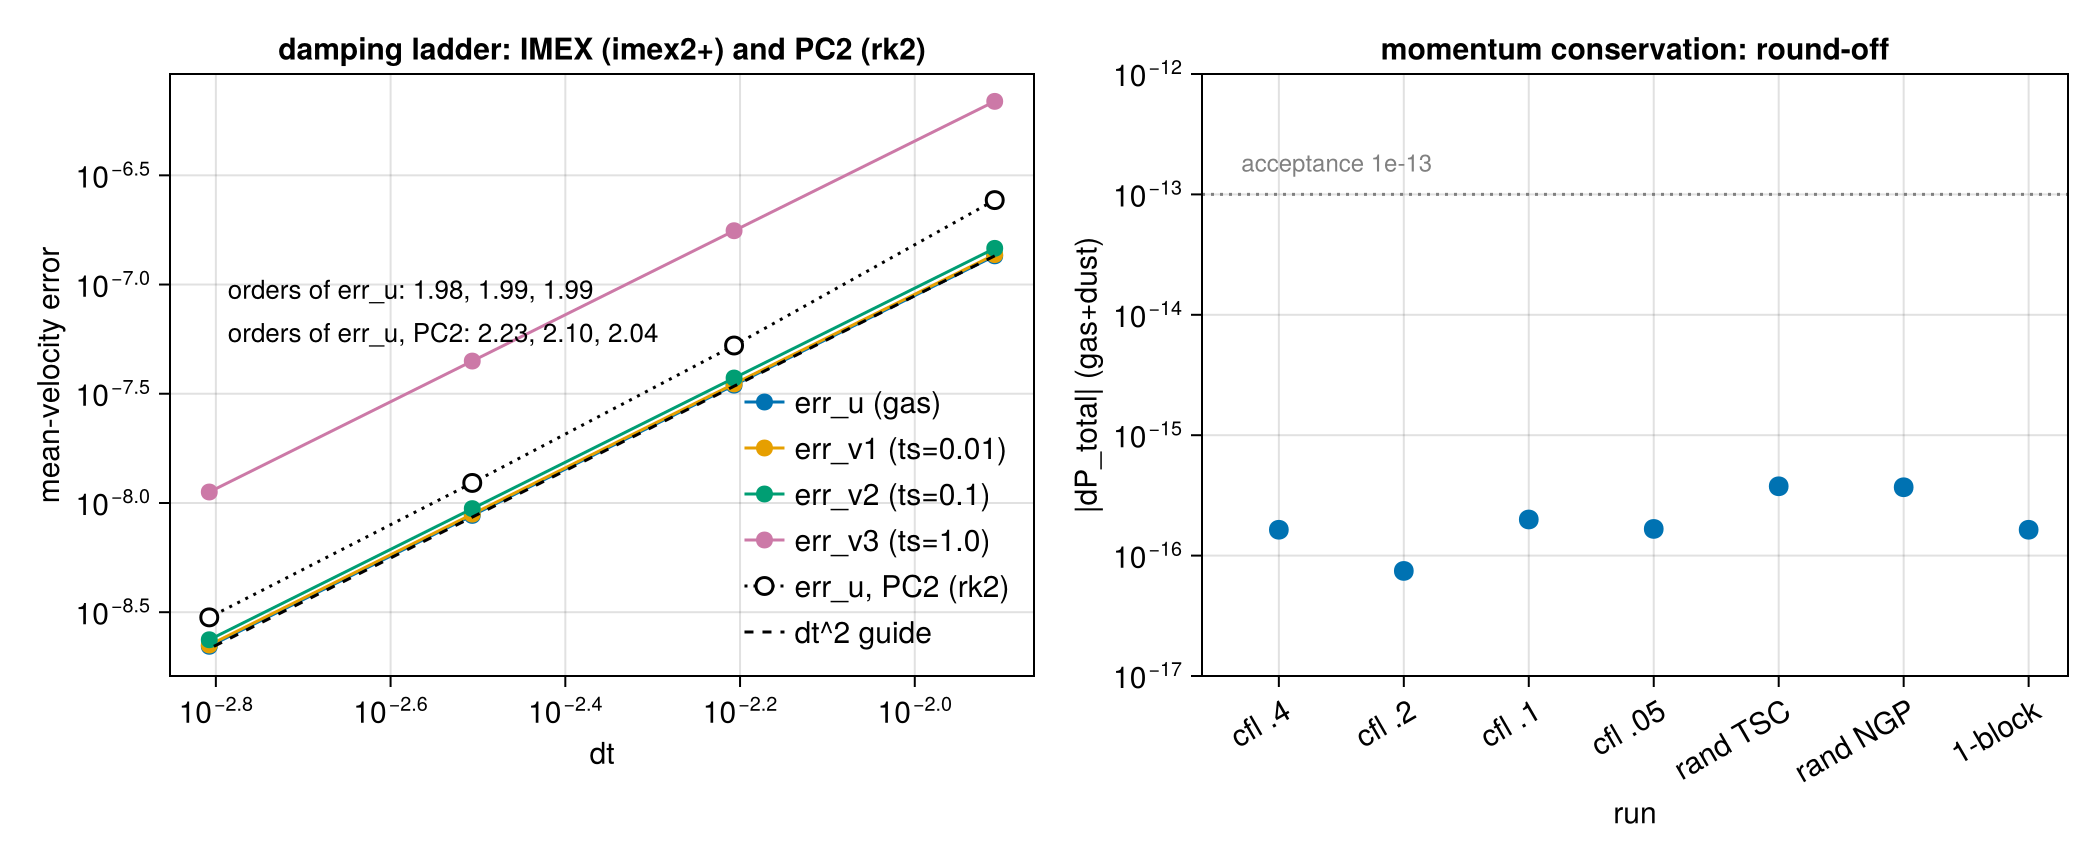
\includegraphics[width=\textwidth]{figures/dust4a_damping.png}
\caption{The damping ladder on the merged tree: second-order convergence of all four
mean-velocity errors in $\Delta t$ under the IMEX coupling (filled), the gas error
under the PC2 coupling with \code{rk2} after the second merge (open, \S\ref{sec:merge2}),
and the total gas$+$dust momentum change of every IMEX run against the $10^{-13}$
acceptance line (right).}
\label{fig:damping}
\end{figure}

\paragraph{NSH drift equilibrium (2D $r$--$z$, ten orbits).} Gas plus three species
($t_s = 0.01, 0.1, 1.0$; $\epsilon = 0.2, 0.5, 0.3$) started at the exact multi-species
steady drift solution, with the gas forced by the pressure-gradient mimic
$2\Om\eta v_K$. After 4495 cycles every deviation is at round-off:

\begin{center}
\small
\begin{tabular}{@{}lcccccccc@{}}
\toprule
 & $|\delta u_x|$ & $|\delta u_\phi|$ & $|\delta v_{x,1}|$ & $|\delta v_{\phi,1}|$ &
   $|\delta v_{x,2}|$ & $|\delta v_{\phi,2}|$ & $|\delta v_{x,3}|$ & $|\delta v_{\phi,3}|$ \\
\midrule
serial & $1.3\times10^{-16}$ & $6.2\times10^{-17}$ & $6.9\times10^{-17}$ & $5.9\times10^{-17}$ &
  $1.2\times10^{-16}$ & $2.4\times10^{-17}$ & $9.4\times10^{-17}$ & $4.3\times10^{-17}$ \\
4 ranks & $1.1\times10^{-16}$ & $9.0\times10^{-17}$ & $1.2\times10^{-16}$ & $2.8\times10^{-17}$ &
  $1.3\times10^{-16}$ & $1.0\times10^{-17}$ & $9.0\times10^{-17}$ & $3.3\times10^{-17}$ \\
\bottomrule
\end{tabular}
\end{center}

This is the test that certifies the rotation/forcing kicks and the implicit drag are
composed unsplit inside the IMEX stages: any splitting error would show as secular
drift.

\paragraph{Damped dusty sound wave (Laibe \& Price 2011; Krapp et al.\ \S3.2).} The
exact complex eigenmode of the linearized gas--dust system, $L_1$ errors of density
and velocity against the analytic damped wave at $t = 2$:

\begin{center}
\small
\begin{tabular}{@{}rcccc@{}}
\toprule
$N_x$ & cycles & $L_1(\delta\rho)$ & $L_1(\delta v_x)$ & order \\
\midrule
32  & 320  & $1.836\times10^{-8}$  & $1.351\times10^{-8}$ & --- \\
64  & 321  & $6.896\times10^{-9}$  & $5.124\times10^{-9}$ & 1.41 \\
128 & 641  & $1.837\times10^{-9}$  & $1.377\times10^{-9}$ & 1.91 \\
256 & 1281 & $4.765\times10^{-10}$ & $3.572\times10^{-10}$ & 1.95 \\
\bottomrule
\end{tabular}
\end{center}

The code's own root of the dispersion relation, $\omega = 4.529763 - 0.492158\,i$,
is printed identically in every run. The order approaches two from below; the
$32 \to 64$ step is polluted by the fixed-\code{cfl} time step at the coarsest
resolution (the same cycle count at 32 and 64 cells), as the dust-tests notebook
also observes.

\subsection{Regressions}

The ion-neutral C-shock (\file{inputs/ion-neutral/perp\_cshock.athinput},
\code{integrator = imex2+}, 500 cycles) is the direct consumer of the refactored
\code{imex2+} coefficient code: RMS-$L_1$ $= 2.071216\times10^{-3}$, bit-identical to
the dust fork's baseline. The Sod tube runs through the untouched hydro task list.

\subsection{Rank independence, and the deadlock}
\label{sec:mpi}

The damping problem with drifting particles (\code{v0 = 0.5}, $t_{s,3} = 0.5$, three
lattice species) sends particles across MeshBlock and rank boundaries many times per
run and exercises per-stage migration, the additive deposit exchange, the $u^\ast$
ghost fill and the back-reaction exchange.

The first attempt at 4 ranks \textbf{hung at cycle 0}. The cause was in the merge
itself: the dust fork's additive deposit exchange posted per-neighbor MPI messages
against the base class of July's upstream, while this tree carries upstream \#775,
whose base-class receive posting is rank-packed (one aggregated message per peer
rank). The sends had no receiver. After moving the exchange onto the rank-packed
path (implementation document \S4.4) with the serial path untouched (the damping
ladder is bit-identical before and after the edit):

\begin{center}
\small
\begin{tabular}{@{}lccccc@{}}
\toprule
ranks & err$_u$ & err$_{v1}$ & err$_{v2}$ & err$_{v3}$ & $|\Delta P_{\rm tot}|$ \\
\midrule
1 & $1.158578\times10^{-5}$ & $1.187422\times10^{-5}$ & $1.490167\times10^{-5}$ & $6.153323\times10^{-5}$ & $5.2\times10^{-15}$ \\
2 & $1.158578\times10^{-5}$ & $1.187422\times10^{-5}$ & $1.490167\times10^{-5}$ & $6.153323\times10^{-5}$ & $3.7\times10^{-15}$ \\
4 & $1.158578\times10^{-5}$ & $1.187422\times10^{-5}$ & $1.490167\times10^{-5}$ & $6.153323\times10^{-5}$ & $3.6\times10^{-15}$ \\
\midrule
reference & $1.158578\times10^{-5}$ & \multicolumn{4}{l}{(dust tests: ``1-rank and 4-rank identical'')} \\
\bottomrule
\end{tabular}
\end{center}

The tiny spread in $|\Delta P|$ is the reduction order of the diagnostic itself. The
NSH run at 4 ranks is in the table of \S\ref{sec:fidelity}.

\subsection{Gravity regression}
\label{sec:gravity}

\begin{center}
\small
\begin{tabular}{@{}>{\raggedright\arraybackslash}p{4.4cm}>{\raggedright\arraybackslash}p{2.6cm}>{\raggedright\arraybackslash}p{4.9cm}>{\raggedright\arraybackslash}p{3.3cm}@{}}
\toprule
test & metric & measured & documented \\
\midrule
\file{mg\_poisson\_slab}, sheet profile (absolute, no mean subtraction) & max rel / $L_2$ rel &
  $1.203474\times10^{-12}$ / $3.078736\times10^{-13}$ & $1.2\times10^{-12}$ \\
\file{ts41\_sin3} (Tomida \& Stone \S4.1) & defect ratio per V-cycle &
  $0.1254$, $0.1249$, $0.1249$, $0.1249$ & $0.125$ \\
\file{mg\_poisson\_shear\_bndry}, shwave, $t_0 = 0.37$ & max rel / $L_2$ rel &
  $5.950118\times10^{-3}$ / $2.057024\times10^{-3}$ & $5.95\times10^{-3}$ / $2.057\times10^{-3}$ \\
same, $t_0 = 0$, shear-periodic vs periodic-$x_1$ twin & both runs &
  $5.506611\times10^{-3}$ / $1.281655\times10^{-3}$, identical & bit-identical \\
\bottomrule
\end{tabular}
\end{center}

At 4 ranks the slab and boundary-annuli solves reproduce the serial digits exactly,
as documented for Phases 2b and 3.

The dust module is inert without a \code{<dust>} block by construction (the hydro
and gravity paths do not see it), and these numbers confirm the shared
infrastructure it touched --- driver coefficients, boundary-values base class,
output tables, physics registration --- left the solver untouched.

\subsection{The integrator twin}
\label{sec:twin}

The Phase-3 small stratified gravito-turbulence box
(\file{inputs/shearing\_box/gravito\_turb\_amr\_test.athinput}: $16H\times16H\times12H$,
$64\times64\times48$, $\beta = 10$, slab-open multigrid gravity, refinement switched off)
evolved to $t = 3\,\Om^{-1}$ with \code{rk2} and with \code{imex2+}, both at
\code{cfl\_number = 0.3}. Relative differences of the history columns at $t = 3$:

\begin{center}
\small
\begin{tabular}{@{}lccccccc@{}}
\toprule
 & mass & $E_{\rm tot}$ & $E_{\rm int}$ & $\langle\rho\,c_s\rangle$ & $\langle\rho\,w_{\rm grv}\rangle$ &
   $\langle\rho\,w_{\rm rey}\rangle$ & $\langle\rho\,\delta v^2\rangle$ \\
\midrule
$|\mathrm{imex2+} - \mathrm{rk2}|/|\mathrm{rk2}|$ & $2.0\times10^{-6}$ & $7.0\times10^{-5}$ &
  $6.3\times10^{-5}$ & $3.5\times10^{-5}$ & $5.3\times10^{-3}$ & $3.2\times10^{-4}$ & $3.2\times10^{-4}$ \\
\bottomrule
\end{tabular}
\end{center}

Two different second-order integrators (three explicit stages of which the first
advances by $\gamma\Delta t \approx 1.71\Delta t$, versus two) on a chaotic flow:
agreement at $10^{-4}$--$10^{-3}$ in the bulk quantities, with the small
gravitational stress --- a difference of large terms at this early time --- the
loosest at $5\times10^{-3}$ (Fig.~\ref{fig:twin}). The spikes of the relative
difference of the stress columns at $t \approx 1.75$ and $2.5$ in the figure are
zero crossings of the stresses themselves (top-left panel), where a relative measure
carries no information. This is the level at which
\code{rk2}-validated gravity results transfer to dust runs; the full-size SC14
statistics under \code{imex2+} are a cluster item and will be attached to the next
$\beta$-scan submission.

\begin{figure}[htbp]
\centering
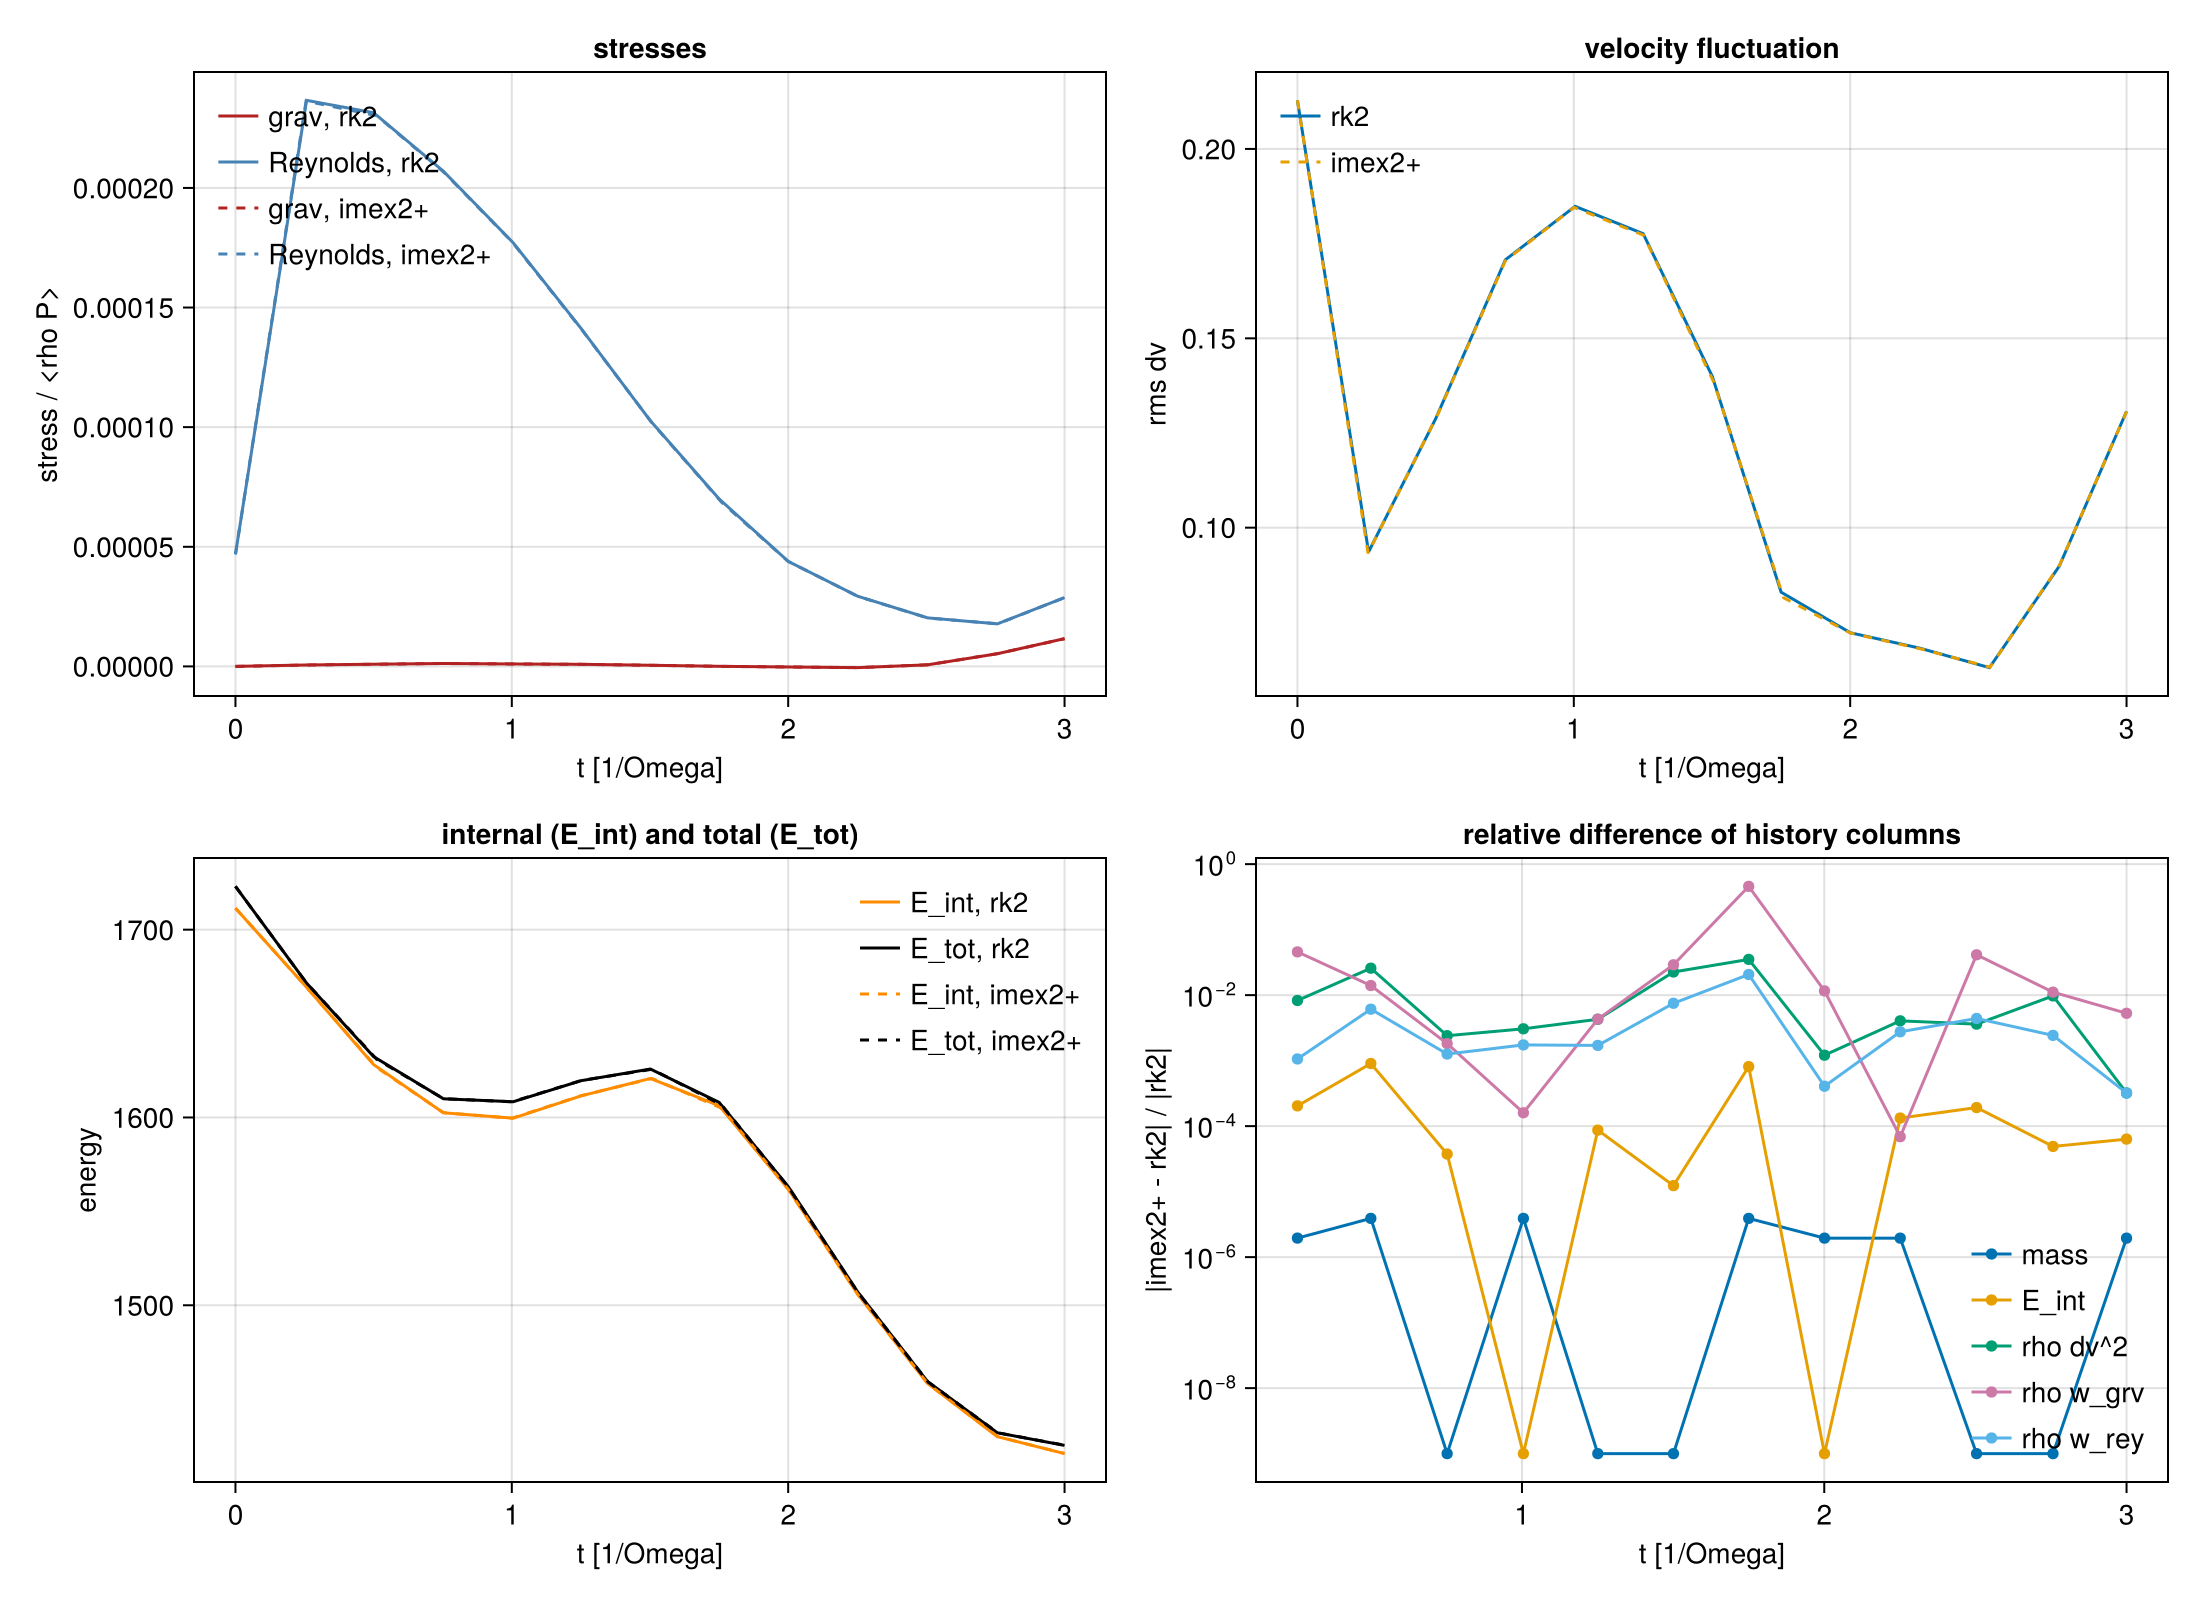
\includegraphics[width=\textwidth]{figures/dust4a_gt_twin.png}
\caption{The gas-only gravito-turbulence box under \code{rk2} (solid) and
\code{imex2+} (dashed): stresses normalized by $\langle\rho P\rangle$, rms velocity
fluctuation, internal and total energy, and the relative difference of the history
columns.}
\label{fig:twin}
\end{figure}

%=========================================================================================
\section{The second merge: regression, and the PC2/hybrid couplings}
\label{sec:merge2}

The dust fork's \code{dust} branch had moved on by seven commits (to \code{1f3e1ed9})
while the first merge was based on \code{d6de1296}; commit \code{78320aee} merges them
(implementation document \S4.5). They bring the fork's own rank-packed deposit
exchange (taken in place of ours), CPU particle-mesh optimizations, and two new
coupling modes selectable with \code{<dust>/coupling}: \code{pc2}, a per-cycle
predictor--corrector particle update under \code{rk2}, and \code{hybrid}, which
switches between PC2 and a first-order split backward-Euler branch on stiffness
measures $\zeta = \max\Delta t/t_s$ and $\chi = \max \Delta t\rho_d/(\rho_g t_s)$.

\subsection{Regression}

Every table of \S\ref{sec:results} was rerun on the rebuilt serial and MPI binaries.
The damping ladder, its three layout variants, the dusty-wave ladder, the C-shock,
the drifting-particle test at 1, 2 and 4 ranks, and all multigrid statics
(serial and 4 ranks) reproduce the printed digits above exactly; the NSH deviations
move within their $10^{-16}$ round-off (the new non-atomic deposit changes the
summation order); and the gas-only gravito-turbulence run is \textbf{bit-identical}
to the pre-merge history, as it must be --- the merge touched nothing on the gas path.

\subsection{PC2 coupling under \code{rk2}}

The inputs are the same test inputs with \code{integrator = rk2} and
\code{coupling = pc2} added to the \code{<dust>} block (archived under
\file{run/dust4a/merge2/}; the key has to be in the file because the command line
cannot add parameters). Damping ladder:

\begin{center}
\small
\begin{tabular}{@{}rccccc@{}}
\toprule
$\Delta t$ & err$_u$ & err$_{v1}$ & err$_{v2}$ & err$_{v3}$ & $|\Delta P_{\rm tot}|$ \\
\midrule
$1.235\times10^{-2}$ & $2.4349\times10^{-7}$ & $2.2596\times10^{-7}$ & $2.4748\times10^{-7}$ & $1.2039\times10^{-6}$ & $2.4\times10^{-16}$ \\
$6.211\times10^{-3}$ & $5.2577\times10^{-8}$ & $4.8577\times10^{-8}$ & $5.3355\times10^{-8}$ & $2.5966\times10^{-7}$ & $4.5\times10^{-17}$ \\
$3.115\times10^{-3}$ & $1.2351\times10^{-8}$ & $1.1216\times10^{-8}$ & $1.2461\times10^{-8}$ & $6.0729\times10^{-8}$ & $5.0\times10^{-17}$ \\
$1.558\times10^{-3}$ & $2.9941\times10^{-9}$ & $2.7081\times10^{-9}$ & $3.0167\times10^{-9}$ & $1.4707\times10^{-8}$ & $5.1\times10^{-17}$ \\
\midrule
order of err$_u$ & \multicolumn{5}{l}{$2.23$, $2.10$, $2.04$ \quad (IMEX ladder: $1.98$, $1.99$, $1.99$)} \\
\bottomrule
\end{tabular}
\end{center}

Second order, converging onto the $\Delta t^2$ slope from above, with errors about
$1.4$--$1.8\times$ the IMEX ones at equal $\Delta t$ and momentum at round-off
(Fig.~\ref{fig:damping}, open markers). The dusty wave:

\begin{center}
\small
\begin{tabular}{@{}rcccc@{}}
\toprule
$N_x$ & $L_1(\delta\rho)$ & $L_1(\delta v_x)$ & order & (IMEX order) \\
\midrule
32  & $1.612\times10^{-8}$  & $1.182\times10^{-8}$  & --- & --- \\
64  & $4.483\times10^{-9}$  & $3.310\times10^{-9}$  & 1.85 & 1.41 \\
128 & $1.139\times10^{-9}$  & $8.404\times10^{-10}$ & 1.98 & 1.91 \\
256 & $2.858\times10^{-10}$ & $2.109\times10^{-10}$ & 2.00 & 1.95 \\
\bottomrule
\end{tabular}
\end{center}

Cleaner second order than the IMEX ladder and smaller errors at every resolution.
The NSH equilibrium under \code{pc2} holds to round-off over the ten orbits
($3.2\times10^{-16}$, $1.3\times10^{-16}$, $3.1\times10^{-16}$, $2.1\times10^{-16}$,
$3.6\times10^{-16}$, $2.4\times10^{-16}$, $1.0\times10^{-17}$, $1.7\times10^{-16}$ for
the eight components of \S\ref{sec:fidelity}). Rank independence with the drifting
particles:

\begin{center}
\small
\begin{tabular}{@{}lccccc@{}}
\toprule
ranks & err$_u$ & err$_{v1}$ & err$_{v2}$ & err$_{v3}$ & $|\Delta P_{\rm tot}|$ \\
\midrule
1 & $6.805779\times10^{-6}$ & $5.812361\times10^{-6}$ & $7.380154\times10^{-6}$ & $3.360985\times10^{-5}$ & $1.5\times10^{-14}$ \\
2 & $6.805779\times10^{-6}$ & $5.812361\times10^{-6}$ & $7.380154\times10^{-6}$ & $3.360985\times10^{-5}$ & $1.9\times10^{-15}$ \\
4 & $6.805779\times10^{-6}$ & $5.812361\times10^{-6}$ & $7.380154\times10^{-6}$ & $3.360985\times10^{-5}$ & $3.9\times10^{-15}$ \\
\bottomrule
\end{tabular}
\end{center}

\subsection{Hybrid coupling and the split-BE branch}

Two runs characterize the fallback. The three-species NSH test under
\code{coupling = hybrid} (automatic selection) reports
\code{pc2\_cycles=0 split\_be\_cycles=4494} with $\zeta = 0.549$: the $t_s = 0.01$
species puts $\Delta t/t_s$ just above the $0.5$ entry threshold, so the run stays
in the first-order branch throughout, and the equilibrium is no longer an exact
fixed point --- deviations of $1$--$12\times10^{-5}$ after ten orbits instead of
round-off. This is the designed behavior, not a defect: the first-order splitting
error of a stiff fallback, on a problem whose IMEX and PC2 answers are exact. The
stiff damping case of the dust tests ($t_s = 10^{-4}, 10^{-3}, 2\times10^{-3}$,
$\Delta t/t_s$ up to $125$) under \code{hybrid} runs split-BE for all 81 cycles
($\zeta = 32.8$, $\chi = 12.6$) and lands on the exact relaxed state
(errors $\le 4.9\times10^{-16}$, momentum $1.1\times10^{-16}$), the L-stability that
the branch exists for. For production runs in the resolved regime the recommendation
is therefore \code{coupling = pc2}; \code{hybrid} is the safety net for
configurations with stopping times below the timestep.

%=========================================================================================
\section{Summary}
\label{sec:summary}

Phase 4a delivers the dust module inside the multigrid tree with both sides
certified unchanged: the dust fork's acceptance numbers and the gravity solver's
documented statics reproduce to every printed digit, serially and at 4 ranks, and
the one merge defect (the additive deposit exchange against rank-packed messaging)
is fixed with a rank-independence table to show for it. The integrator the
dust module's IMEX coupling imposes, \code{imex2+}, tracks \code{rk2} on the stratified
gravito-turbulent box at the level two second-order schemes should --- and after the
second merge that constraint is optional: the PC2 coupling runs under \code{rk2} at
second order with the same conservation properties, and is the recommended
production path in the resolved drag regime.

What 4a does \emph{not} yet provide, and Phase 4b takes up next: the shear-periodic
remap of the additive deposits (the module warns that ghost deposits cross the
radial faces unremapped, exact only for axisymmetric states), back-reaction with an
ideal-gas energy equation (required for cooling), and a particle timestep that does
not pay the full-shear-velocity penalty in wide boxes. The tests for those are the
3D shear-periodic NSH state, an azimuthally structured deposit conserved through the
remap, and the momentum--energy budget of a drag-coupled ideal gas.

\end{document}
